\section{Image classification}
\label{sec:cnn}

In this section, we will learn how to conduct computational image classification which is probably the most extended supervised machine learning application in the field of automatic analysis of images in communication and social sciences. We will firstly discuss how to apply a \textit{shallow} algorithm and then a deep-learning approach, given a labelled data set. 	

In an image classification task we train a model with examples (e.g. a corpus of pictures with labels) in order to predict the category of any given new sample. It is the same logic used in supervised text classification  explained in Section~\ref{sec:supervised} but suing images instead of texts. For example, if we show many pictures of cats and many of houses the algorithm would learn the constant features in each and will tell you with some degree of confidence if a new picture contains either a cat or a house. It is the same with letters, numbers, objects or faces, and you can apply either binary or multi-class classification. Just think when your vehicle registration plate is recognized by a camera or when your face is automatically labelled in pictures posted in Facebook.

Beyond image classification we have other specific tasks in computer vision such as \textit{object detection} or \textit{semantic segmentation}. To conduct object detection we have first to locate all the possible objects contained in a picture by predicting a bounding box (i.e. height and weight, as well as the four points corresponding to the vertical and horizontal coordinates of the center of the object), which is normally an regression task. Once the bounding boxes are placed around the objects, we must apply multi-class classification as explained earlier. In the case of semantic segmentation, instead of classifying objects, we classify each pixel of the image according to the class of the object the pixel belong to, which means that different objects of the same class might not be distinguished. Figure~\ref{fig:location} shows an example of each of these techniques presented by \citet{geron2019hands}.

\begin{figure}
\centering
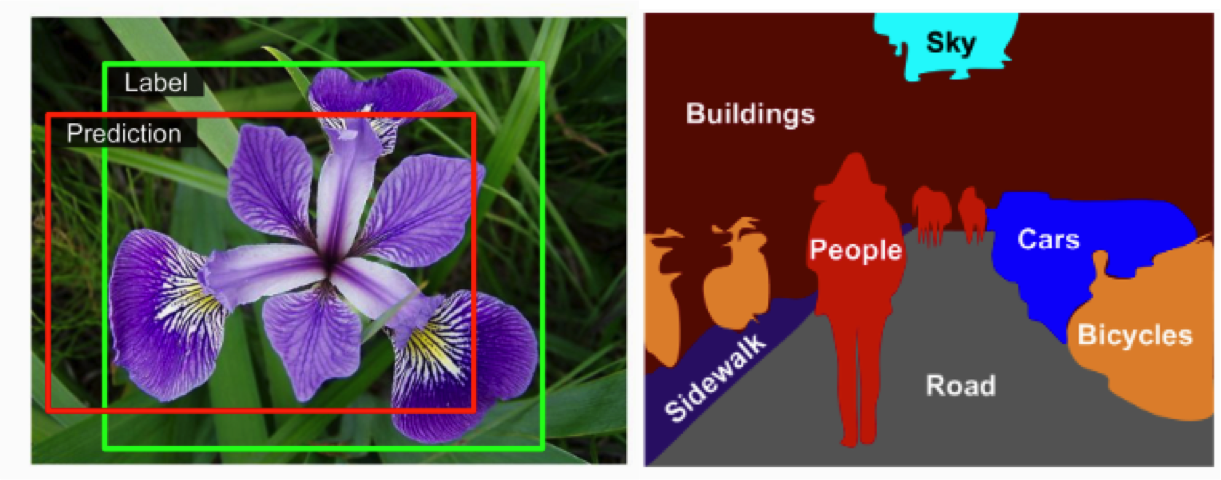
\includegraphics[width=0.9\linewidth]{figures/ch15_location.png}
\caption{Object detection (left) versus semantic segmentation (right).
Source: \citet{geron2019hands}}
\label{fig:location}
\end{figure}

It is beyond of the scope of this book to address the implementation of object detection or semantic segmentation, but we will focus on how to conduct basic image classification in state-of-the-art libraries in R and Python. As you may have imagined we will need some already-labelled images to have a proper training set. It is also out of the reach of this chapter to collect and annotate the images, which is the reason why we will mostly rely on pre-existing image databases (i.e. MINST or Fashion MINST) and pre-trained models (i.e. CNNs architectures), or will provide you with ad hoc annotated images if it is necessary. 

\subsection{Basic classification with shallow algorithms}
\label{subsec:shallow}

In Chapter~\ref{chap:introsml} we introduced you into the exciting world of machine learning and in Section~\ref{sec:supervised} we showed how to used the \textit{supervised} approach to classify texts. Most of the discussed models were based in the so called \textit{shallow} algorithms (Naïve Bayes, Regression, Support Vector Machines, Decision Trees or Random Forest), in opposition to other algorithms liked to \textit{deep} learning. As we will see in the next section, deep neural networks are nowadays the best option for complex tasks in image classification. However, we will now explain how to conduct simple multi-class classification of images that contain numbers with some shallow algorithms.

Let us begin by training a model to recognize numbers using 70,000 small images of digits handwritten from the Modified National Institute of Standards and Technology (MNIST) dataset  (\cite{lecun1998gradient}). This popular training corpus contains gray-scale examples of numbers written by American students and workers and it is usually employed to test machine learning models (60,000 for training and 10,000 for testing). Image sizes are 28 x 28, which generates 784 features for each image, with pixels values from white to black represented by a 0-255 scales. In Figure~\ref{fig:numbers} you can observe the first 10 handwritten numbers used in both training and test set.

\begin{figure}
\centering
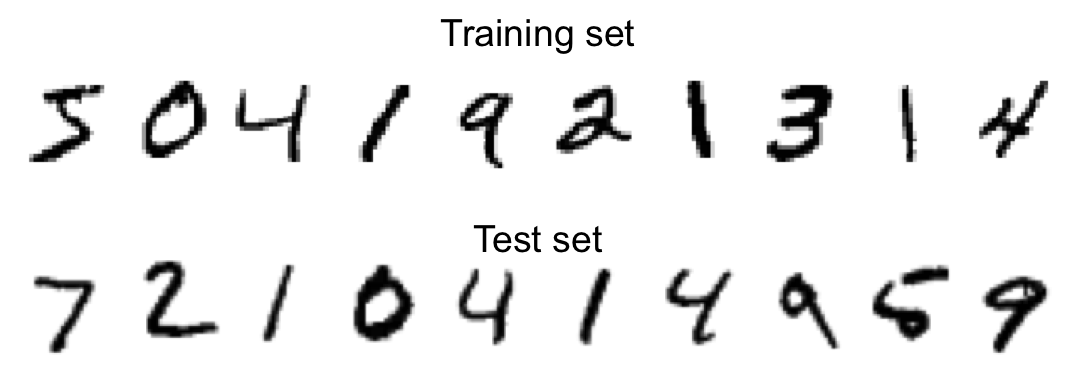
\includegraphics[width=0.9\linewidth]{figures/ch15_numbers.png}
\caption{First 10 handwritten digits from the training and test set of the MNIST}
\label{fig:numbers}
\end{figure}

You can download the MNIST images from its project web page\footnote{http://yann.lecun.com/exdb/mnist/}, but many libraries also offer this dataset. In \refex{mnist} we use the \fn{read\_mnist} function from the \pkg{dslabs} package (Data Science Labs) in R and the \fn{fetch\_openml} function from the \pkg{sklearn} package (\texttt{datasets} module) in Python to read and load a \texttt{mnist} object into our workspace. We then create the four necessary objects (\texttt{X\_train}, \texttt{X\_test}, \texttt{y\_train}, \texttt{y\_test}) to generate a ML model and print the first numbers in training and test sets and check they coincide with those in \ref{fig:numbers}.

\pyrex[output=both,caption=Loading MNIST dataset and preparing training and test sets]{chapter15/mnist}

Once we are ready to model the numbers we choose one of the shallow algorithms explained in Section \ref{sec:nb2dnn} to deploy a binary or multiclass image classification task. In the case of binary, we should select a number of reference (for instance "3") and then create the model of that number against all the others (to answer questions such as "What's the probability of this digit of being number 3?). On the other hand, if we choose multiclass classification our model can predict any of the ten numbers (0, 1, 2, 3, 4, 5, 6, 7, 8, 9) included in our examples.

Now, we used the basic concepts of the Random Forest algorithm (see subsection~\ref{subsec:randomforest}) to create and fit a model with 100 trees (\texttt{forest\_clf}). In \refex{multiclass} we use again the \pkg{randomForest} package in R and \pkg{sklearn} package in Python to estimate a model for the ten classes using the corpus of 60,000 images (classes were similarly balanced (~9-11\% each). As we do in the examples, you can check the predictions for the first ten images of the test set (\texttt{X\_test}), which correctly correspond to the right digits, and also check the (\texttt{predictions}) for the whole test set and the some metrics of the model. The accuracy is over 0.97 which is a good indicator in the classification task.

\pyrex[output=both,caption=XXX]{chapter15/multiclass}

This approach based on shallow algorithms seems to work pretty well for simple images, but has a lot of limitations for more complex images such as figures or real pictures. In the next section we introduce the use of deep learning in image classification which is nowadays a more accurate approach for complex tasks.


\subsection{Deep learning for image analysis}
\label{subsec:deep}

MLP for image classification p 297   Fashion MNIST (https://github.com/zalandoresearch/fashion-mnist)

\subsection{Fine tuning an open source CNN}
\label{subsec:deep}

Fine tuning an open source CNN   RestNet 18? (Andreu example)